%----------------------------------------------------------------------------------------
%	PACKAGES AND OTHER DOCUMENT CONFIGURATIONS
%----------------------------------------------------------------------------------------

\documentclass[12pt]{report} 
% Default font size is 12pt, it can be changed here

\usepackage{appendix}
\usepackage{geometry} % Required to change the page size to A4
\geometry{a4paper} % Set the page size to be A4 as opposed to the default US Letter

\usepackage{graphicx} % Required for including pictures

\usepackage{listings}

\usepackage{cleveref}

\usepackage{tikz}

\usepackage{float} % Allows putting an [H] in \begin{figure} to specify the exact location of the figure
\usepackage{wrapfig} % Allows in-line images such as the example fish picture

\usepackage{lipsum} % Used for inserting dummy 'Lorem ipsum' text into the template

\linespread{1.2} % Line spacing

%\setlength\parindent{0pt} % Uncomment to remove all indentation from paragraphs

\graphicspath{{Pictures/}} % Specifies the directory where pictures are stored

\begin{document}

%----------------------------------------------------------------------------------------
%	TITLE PAGE
%----------------------------------------------------------------------------------------

\begin{titlepage}

\newcommand{\HRule}{\rule{\linewidth}{0.5mm}} % Defines a new command for the horizontal lines, change thickness here

\center % Center everything on the page

\textsc{\LARGE Vrije Universiteit Brussel}\\[1.5cm] 
\textsc{\Large Operating Systems and Security}\\[0.5cm] 
\textsc{\large Mini-project essay}\\[0.5cm] 

\HRule \\[0.4cm]
{ \huge \bfseries High availability and scalability on GNU/Linux clusters}\\[0.4cm] % Title of your document
\HRule \\[1.5cm]

\begin{minipage}{0.4\textwidth}
\begin{flushleft} \large
\emph{Author:}\\
Pieter \textsc{Libin} % Your name
\end{flushleft}
\end{minipage}
~
\begin{minipage}{0.4\textwidth}
\begin{flushright} \large
\emph{Professor:} \\
Prof. Dr. \\Martin \textsc{Timmerman} 
% Supervisor's Name
\end{flushright}
\end{minipage}\\[4cm]

{\large \today}\\[3cm] % Date, change the \today to a set date if you want to be precise

%\includegraphics{Logo}\\[1cm] % Include a department/university logo - this will require the graphicx package

\vfill % Fill the rest of the page with whitespace

\end{titlepage}

\newcounter{treeline}

\newcommand{\treeroot}[1]{% Title
\node[above] at (0,0) {#1};%
\setcounter{treeline}{0}
}

\newcommand{\treeentry}[2]{% Title, Level
\draw[->] (#2-1,-\value{treeline}/2) -- (#2-1,-\value{treeline}/2-0.5) -- (#2+0.5,-\value{treeline}/2-0.5) node[right] {#1};
\stepcounter{treeline}
}

\newcommand{\altentry}[2]{% Title, Level
\draw[->] (#2-1,-\value{treeline}/2) -- (#2-1,-\value{treeline}/2-0.5) -- (#2+0.5,-\value{treeline}/2-0.5) node[right] {#1};
\foreach \x in {1,...,#2}
{   \draw (\x-1,-\value{treeline}/2) -- (\x-1,-\value{treeline}/2-0.5);
}
\stepcounter{treeline}
}

%----------------------------------------------------------------------------------------
%	TABLE OF CONTENTS
%----------------------------------------------------------------------------------------

\tableofcontents % Include a table of contents

\newpage % Begins the essay on a new page instead of on the same page as the table of contents 

\chapter{Introduction} % Major section

\chapter{General scope of availability and scalability}

\chapter{Different aspects in cluster availability}
\label{chap:aspects}
\section{Hardware}
\subsection{Servers}
\subsection{Network}
\subsection{Storage}
also backup devices
\section{Infrastructure}
\subsection{Sites}
\subsection{Buildings}
\subsection{Energy providers}
\section{Internet Availability}
\section{Storage}
http://www.tldp.org/REF/INTRO/Backup-INTRO/strategies.html
http://www.freebsd.org/doc/handbook/backup-strategies.html
\section{Database systems}
traditional vs NOSQL
\section{Application crashes}
\section{Human error}
\section{Operating systems}
microkernel vs monolithic kernels
minix: driver reincarnation
\section{Monitoring}
\section{Virtualization}
\section{Different kinds of outages}
describe types + explain how to measure
\section{Definition of high availability, expectations and realistic
  goals}
99.9999... perc rule

\chapter{Scalability and its effects on economy and environment}

\chapter{Identifying high availability and scalability solutions}
\section{Cluster nodes}
\subsection{Cluster node monitoring}
The two major monitoring tools on GNU/Linux platforms are Nagios and
Ganglia. Both tools implement several monitoring aspects, but the
focus of each of the tools is different. Nagios is more oriented
towards detecting system problems and sending out notificiations for
such events, while Ganglia provides a long term overview of the status
of cluster nodes. To ensure high availability, detecting problems is
the most important aspect. The sooner problems are revealed, the
sooner actions can be undertaken to avoid any impact on end users. It
is imporant that problems are properly communicated to system
administrators, since they might be able to further investigate the
problem. In the event of any hardware failure the intervention of
an administrator will be required. However, it is also necessary that
 it is possible to execute programs repair the state of the cluster
 upon the detection of failure. Nagios specializes on both these
 issues \cite{nagios:2013}.
In order to make new nodes available when necessary, we need to
monitor the resource availability on all of the online nodes.
Monitoring statistics also allows system engineers to gain insight in
performance needs of an application over the course of time. 
Such statistics can also be used to setup models that can be used to
predict system load \cite{andreolini:2006}. Ganglia collects these
kind of statistics and stores them in a round-robin database, namely RDDTool
\cite{ganglia:2013} \cite{rrdt:2013}.
Nagios is free software (GPL) and Ganglia's source code is licensed
under the BSD license. Note that there also exists a commercial
version of the Nagios software: Nagios XI. Nagios XI extends the free
software edition by providing a richer and more powerfull web interface.

\section{Computational cluster nodes}
\subsection{Application monitoring}
Monitoring a cluster node is not enough to garantee that it is
properly servicing clients. It is possible that the application (for
example: the web application server) has gotten in an infinite loop,
and as such is using practically all CPU, but in reality is
processing no new client request.
A possibility to monitor applications is to keep track of the number of
client request per seconds (or another appropriate time unit) that get
processed and compare it with the amount of computational resources
that is used.
This number of client requests is very application specific; a web
server might process thousands client requests per second, while a
server responsable for rendering a scene in an animated movie might only process
one request per hour \cite{apm:2013}.
This information usually can be extracted from the log files generated
by the server application (for example: the request log file for
Apache httpd). This information than can be pass to Ganglia to be
stored and monitored together with the other server's statistics
\cite{ganglia:2013}.

\subsection{Cluster node management}
In large cluster environments, it is not possible to wait for
a human intervention when a problem occurs. Therefore, when nodes or
applications fall away, the monitor server should restart them.
There are several systems that allow for programs to restart
physical servers that reside in a rack (for example Dell's DRAC).
Since I will only use a simulated cluster in this mini-project, I will
only deal with starting and stopping virtualized nodes (which I think should
be a valuable contribution taken into account the large amount of
virtualized server that are used in datacenters these days).
I will use VirtualBox to set up my simulated cluster, this
virtualization software has support to start and stop virtual machines
using the command line.
When an application stalls but the operating system is still fully
functioning, the monitoring server can decide to restart the server application, or
(if the application has support for this) simply kill the thread that
is responsible for the problems.

\subsection{Load balancing proxies}
\label{sec:load_balancing_proxies}
Load balancing is a method for distributing workloads across multiple
computing nodes. It can be used to improve the reliabilty of a system through
redundancy and to provide scalability by sending requests the most
available node.
Load balancing has several applications such as High Performance
Clusters, database servers, and HTTP servers. In this section I will
focus on HTTP load balancing.
A prominent TCP/HTTP load balancing proxy is HAProxy.
\cite{haproxy:2013}. HAProxy is free software (GPLv2 for most of the
code, LGPLv2 for some of the headers). This software supports a set of
balancing algorithms \cite{tarreau:2006}, most notably:
\begin{itemize}
  \item round robin: each server is used in turns, taking into account
    the different server's weights (these weights can be configured
    per server and can be adjusted on the fly)
  \item balance leastconn: the server with the lowest number of connections receives the connection
  \item source/uri: this algorithm hashes respectively the source IP
    or URI of the request, this hash is than divided by the total
    weight of the running servers to determine which server should
    receive the request
\end{itemize}
HAProxy also supports Access Control Lists configurations that allow
the load balancer to select a server based on a header in the HTTP
request. When multiple server clusters exists in different countries
and/or continents, this feature allows us to connect a user to a
server that is located near his own location.
Another important aspect to consider when setting up a load balancing
infrastructure for HTTP servers is that many dynamic web applications
rely on session context \cite{tarreau:2006}. Since this session context is usually stored
on the web server, it is necessary for the load balancer to pass the
client's request to the same web server: this is called persistence.
HAProxy provides session context persistence through `cookie
learning' or `cookie insertion'. When using `Cookie learning' the load
balancer will store a connection between an appliction cookie (this
application cookie has to be configured) and a server. The
disadvantages of this approach are:
\begin{itemize}
  \item the application cookie -> server mapping requires memory
  \item if the load balancer crashes, there is no way to connect the
    client back to the server
\end{itemize}
`Cookie insertion' avoids these problems by adding a cookie that
identifies the server to the response that is sent to the client. By
using this approach the load balancer can simply reuse the
cookie value presented by the user to pass the request to the correct
server.

\section{Storage and backup}

\subsection{Data replication}
Data replication implies that the same date is stored on multiple
data storage systems. This should be transparant to the end user: the
user should not be aware of this when using the data (note that when
working with a multi-tier architecture, it is possible that the
`end-user'  is represented by another tier in the system).
Data replication is relevant for both:
\begin{itemize}
\item high availability systems: to ensure a smooth transition from a
  failing data storage node to a working node
\item systems that require scalability: to make load balancing possible
\end{itemize}
We can distinguish 3 types of data replication
\cite{datareplication:2013} :

\subsubsection{Database replication}

\paragraph*{Master-slave replication}
In this setup, there exists one master database, this database is the only instance
that accepts updates. When an update statement is received by the
master database, it is applied to the database and appended to the log. The statements
in this log are than propagated to the slave databases.
Most database systems support this replication strategy (Postgres \cite{postgres_db:2013},
MySQL \cite{mysql_db:2013}, ...).
Mention uses:
- backup of database
- use a slave database without causing load on the master (statistics
for example)
- scale out: for read only access, let a proxy determine which slave
needs to be used

\paragraph*{Multi-master replication}
In this setup, multiple master instances exists, each of these master
instances accept updates. These updates are than communicated with the
other master instances. 
This has the advantages that :
\begin{itemize}
\item the master node can fail without interrupting the system
\item the update load can be distributed over multiple nodes
\end{itemize}
There are also some significant disadvantages related to this technique:
\begin{itemize} 
\item increased complexity
\item most implementations violate the ACID constraints
\item to fix conflicts that may arise between different database
  instances, resources of the database nodes are required and
  communication between the conflicted nodes will increase the network
  traffic
\end{itemize}
Note that there are other techniques to accomodate the advantage of
load balancing mentioned above: database shards, NoSQL (reference to
this section).

\subsubsection{Disk storage replication}
Disk storage replication collects updates to a block device and
applies these updates collectively to multiple devices.
This can be implemented in hardware, the functionality is than
embedded in the array disk controller (RAID-1).
DRBD \cite{drbd_soft:2013} implements this functionality in software.
This software allows users to mirror disks within a system or over a
network (the DRBD website explains this as follows: ``DRBD can be
understood as network based raid-1'' \cite{drbd_soft:2013}).

\subsubsection{File-based replication}
Disk storage replication replicates entire block devices, however for
some applications, it might be necessary to only replicate parts of
the logical file system.
\paragraph*{Batch replication}
To replicate file systems in batch, synchronization tools such as
rsync \cite{rsync_software:2013} can be
used. The rsync Unix tool can synchronize 2 directories from one location to the
other (this can be done over a network). The advantage compared to a
simple ``scp -r'' is that rsync will only transfer the changes by using
delta encoding.
\paragraph*{Real-time replication}
I was not able to find any tools on GNU/Linux that allow real-time
file-based replication based with default filesystems such as ext4.
It is however possible to achieve this kind of file-based replication
by using one of the distributed file systems, which I will discuss in
the next section.

\subsection{Backup}
Different backup strategies were discussed in 
\cref{chap:aspects}, some of these strategies require methods of data
replication (as discussed in the previous section).
In order to setup a reliable backup system, some other technologies
are required: 
\begin{itemize}
\item the ability to take a snapshot of a file system: this can be
  achieved by using the Logical Volume Manager, which is part of the
  mainline Linux kernel \cite{linux_kernel_soft:2013}
\item the ability to take snapshots and incremental backups of RDBMs: most RDBMS systems
  support this; some examples:
  \begin{itemize}
  \item Postgres: via barman \cite{barman_software:2013}
  \item MySQL: via mysqldump (and by enabling the binary log)
  \end{itemize}
\item the ability to make incremental filesystem backups; this can be
  done using rsync \cite{rsync_software:2013}
\end{itemize}
\subsection{Distributed file systems}
Distributed file systems share storage using a network protocol, they
deliver scalability and failure
correction in such a way that it is transparent to the client.
Such filesystems can restrict access to certain files based on access lists
and/or file system quotas. Distributed file systems allow clients to
access files in the same way as they would be able to do on their
local file system (note that a client might refer to an end user, 
but it might as well refer to one of the tiers in a multi-tier
system).
The most interesting free software implementations I encountered were
GlusterFS \cite{glusterfs_soft:2013} and Ceph \cite{ceph_soft:2013}
(which also is a object and block storage system).

\section{Databases}
\section{RDBMS sharding}
For some application, the amount of data that needs to be stored can be so high
that it is impossible to fit it on a single cluster node. In order to
accomodate such large database in a relational context, database
sharding can be used. Database sharding allows databases to be
partioned horizontally; so that different rows of the database can
reside on different cluster nodes. It is advisable that rows that are
closely connected are located on the same cluster node, to improve
query performance, however, it still remains possible to execute
queries that involve rows distributed over multiple cluster nodes.
For example: an application where the data that is stored is mostly 
private to a user (storage of emails, storage of Skype contacts, ...),
 could be sharded by the user name.
Both MySQL \cite{mysql_db:2013} and Postgres \cite{postgres_db:2013}
support database sharding.
\section{Document-oriented NoSQL databases}
When the data that is stored is private to one user and performing
queries over multiple users is a rare event (storage of emails,
storage of Skype contacts, ...), it can be interesting to keep a
database per user. This can be achieved by using so-called
document-oriented NoSQL solutions. 
These solutions are able to store a document
containing all information related to one user. This document can for
example be structured using the JSON format. Contrary to RDBMS
systems; document-oriented NoSQL solutions have no schemas that define
how the data should be structered, instead fields can be freely added
to the JSON documents.
Altough this provides a greater flexibility, this also makes it very
difficult to perform queries over multiple documents that require data
to be joined together.
When data is grouped together in a document per entity (e.g.: a user)
and this document is stored in one file; it becomes much easier to scale the data over
multiple clusters.
With the booming of the ``cloud'' several document-oriented NoSQL
solutions have been developed, most notably: CouchBase and MongoDB.

\chapter{Experimenting with HA and scalability solutions}
\section{Open source technologies}
Focus on open source technologies. ... 

\section{Test environment setup}
I will simulate a mini-cluster using different virtual machines. I
will create these virtual machines with VirtualBox
\cite{virtualbox_soft:2013}.  The virtual machines will have
``Ubuntu Linux 13.10 (AMD64) Server Edition''
\cite{ubuntu_server_13_10:2013} installed as base operating system.

I want all the virtual machines to be able to contact each other,
while it should also be possible for them to access
the internet.
To make this possible, I opted to use the virtualized NAT
VirtualBox feature (this is a new feature, available since version
4.3).
This new feature emulates a NAT environment on your host machine.
The advantage of this is that the test setup will also work when no
network is available.

Created base VM, to be cloned...
Shared filesystem: to allow automatic mounting -> guest additions.
To allow other users to acces this directory, add them to the vboxsf group.


\noindent First we need to create the NAT network:
\begin{lstlisting}[language=bash]
 VBoxManage natnetwork add -t nat-int-network -n "192.168.15.0/24"
                                               -e -h on
\end{lstlisting}
This commands creates the NAT network 'nat-int-network' with an IP
address range between 192.168.15.0/24.
After creating the NAT network, virtual machine guests can be
configured as shown in ~\cref{fig:vbox_network_config}.
\begin{figure}[h!]
  \caption{VirtualBox network configuration.}
  \label{fig:vbox_network_config}
  \centering
    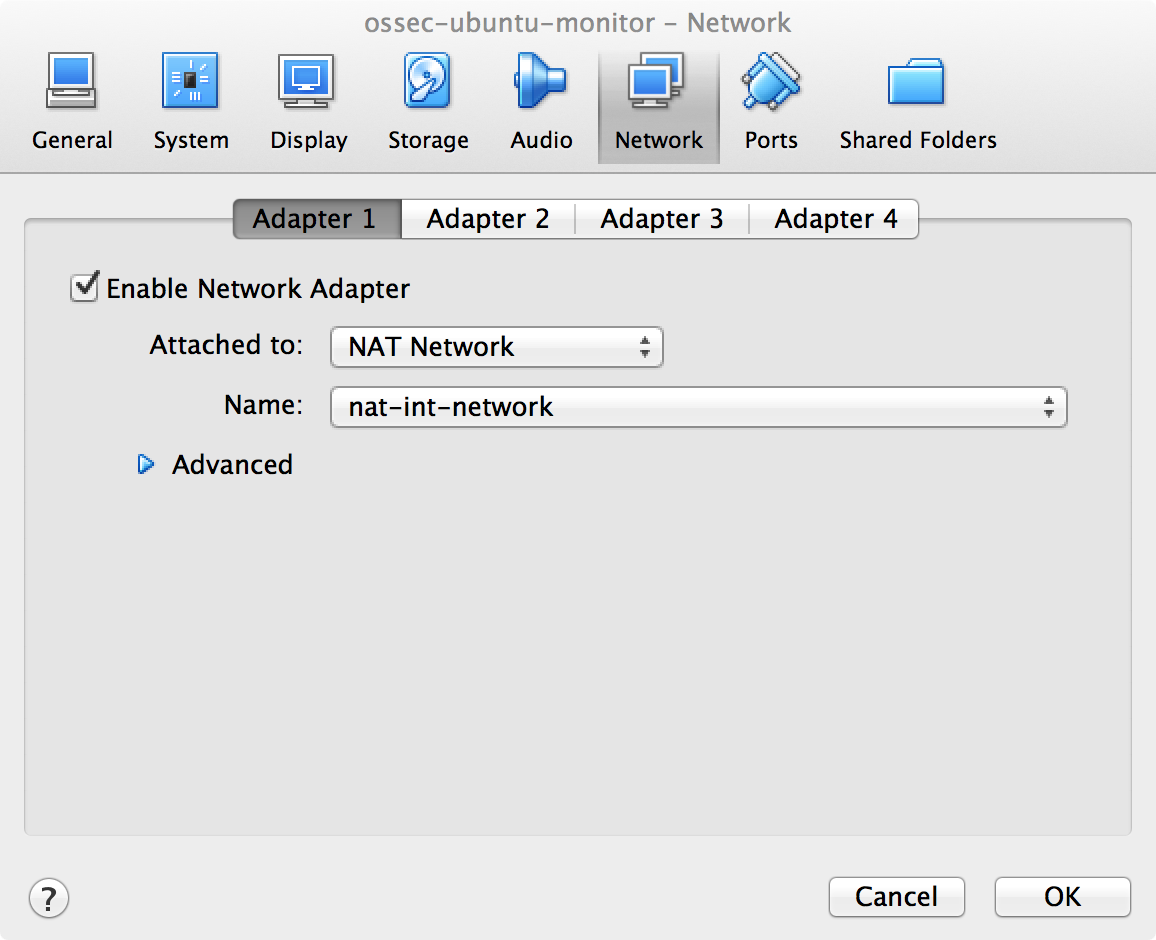
\includegraphics[width=0.5\textwidth]{pics/vbox_network_config.png}
\end{figure}

There was a problem with the system clock on the virtual machines, 
I was able to fix this problem by installing the VirtualBox guest
additions.
Installing guest editions:
-install build-essential
-run script of vbox

\section{Monitoring}
\subsection{Experiment overview}
To test nagios \cite{nagios:2013}, I will test the detection of
application and system failure. To test the application failure, I
will write an example application that fails after
2 minutes. I will test the system failure by inducing a kernel panic.
When an application failure is detected I will execute a script on the
cluster node to restart the application.
When a system failure is detected, I will restart the virtual
machine. 

\subsection{Nagios experiment}
I cloned the base virtual machine as described earlier and changed its
hostname to 'monitor' (by editing $/etc/hostname$ and $/etc/hosts$ and
rebooting). (also mention this for the nodes???)


On this machine, I installed nagios:
\begin{lstlisting}[language=bash]
 sudo apt-get install nagios3
\end{lstlisting}
During this installation a couple of questions were asked:
\begin{itemize}
\item email configuration: since I will not use this in my experiment
  I did not provide a configuration 
\item the nagios web administration password
\end{itemize}
In order to be able to access the web server, I opened port 80 of the
machine's firewall. 
I first enabled the UFW firewall:
\begin{lstlisting}[language=bash]
  sudo ufw enable
\end{lstlisting} 
Then I opened port 80:
\begin{lstlisting}[language=bash]
  sudo ufw allow 80/tcp
\end{lstlisting} 
Since the NAT network setup does only allow virtual machines to access
other virtual machines, I started my Windows virtual machine and used
the web browser to access the nagios system. After providing the
username and password, the browser showed the unconfigured website as
depicted in \cref{fig:nagios_1}.

\begin{figure}[h!]
  \caption{Nagios start page, immediately after installation.}
  \label{fig:nagios_1}
  \centering
    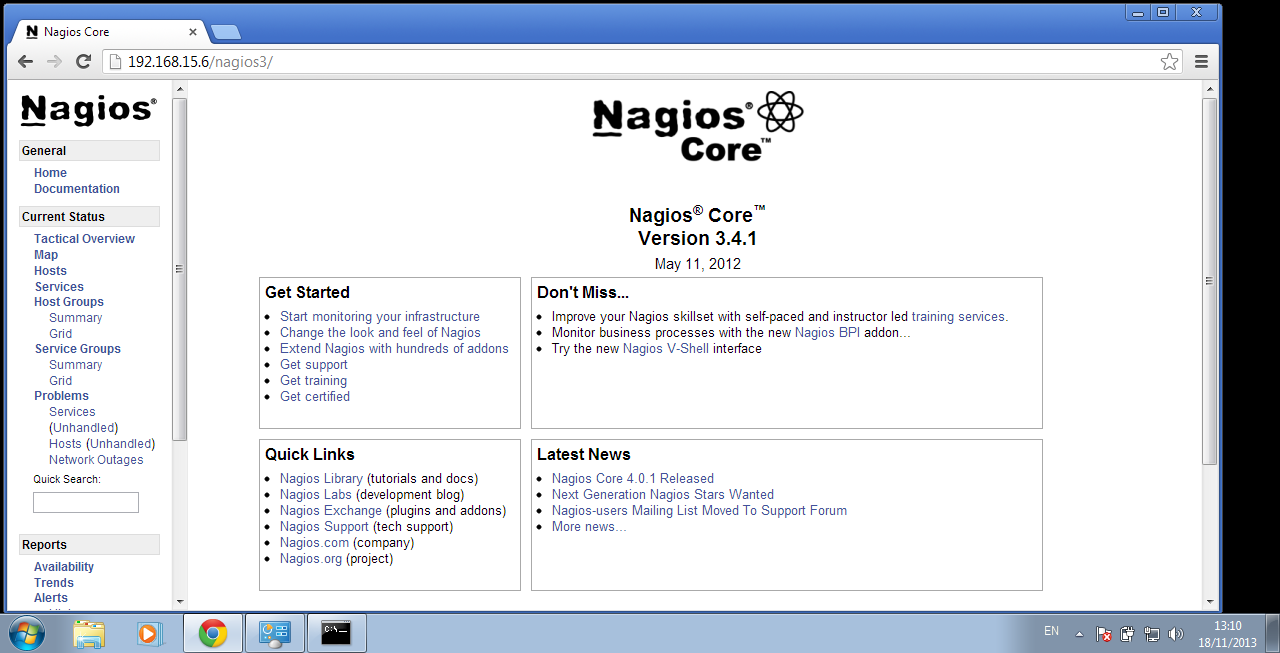
\includegraphics[width=0.5\textwidth]{pics/nagios_1.png}
\end{figure}

I cloned another pair of servers: node1 and node2, that will serve as
cluster nodes.

To test the detection of application failure, I wrote a program that
fails after 2 minutes. As described in the previous chapter, failure
cannot simply be defined as ``using all system resources'', since it
is possible that the server is simply under heavy load. We need to
look at the ratio of $\frac{number of processed items}{usage of system
resources}$. Our test program logs a large number of (fake) transactions per
second while using most of the CPU resources, and after 2 minutes
stops generating transactions, after this point the program will solely occupy CPU
resources (this event defines our failure).

The source code of this program can be found in ... $(nagios\_app.cpp)$
I install it on node1 simply by building the source code:
\begin{lstlisting}[language=bash]
  g++ nagios_app.cpp -o nagios_app 
\end{lstlisting} 
After building the application, I copy it to $/usr/sbin/$.
Note: in order to build this C++ code, we need gcc, this is included
in the package build-essential, which was installed earlier. 

In order to start/stop and restart the service, I create an init.d
configuration script.
I based this script on the code I found on this website: 
http://koo.fi/blog/2013/03/09/init-script-for-daemonizing-non-forking-processes/
I added the source code of the nagios\_app init.d config script $(at src/init.d/nagios\_app)$.
Now we still need to give the script the correct permissions:
\begin{lstlisting}[language=bash]
  sudo chmod 755 /etc/init.d/nagios_app
\end{lstlisting} 
And we need to include it in the startup list:
\begin{lstlisting}[language=bash]
  sudo update-rc.d myscriptname defaults
\end{lstlisting}

We now can start/stop the program very easily:
\begin{lstlisting}[language=bash]
  sudo /etc/init.d/nagios_app start
  sudo /etc/init.d/nagios_app stop
\end{lstlisting}

To monitor a remote server I use the NRPE plugin for Nagios. 
This can be easily installed on the server using this command:
\begin{lstlisting}[language=bash]
  sudo apt-get install nagios-nrpe-plugin
\end{lstlisting} 

To allow nagios to detect the installation of the plugin, we need to
restart apache:
\begin{lstlisting}[language=bash]
  sudo /etc/init.d/apache2 restart
\end{lstlisting} 

On the server that is to be monitored (node1), we need to install the NRPE
deamon, so that the Nagios server can communicate with the remote
server
\begin{lstlisting}[language=bash]
  sudo apt-get install nagios-nrpe-server
\end{lstlisting} 

We can check whether the NRPE plugin can connect to node1, with this command:
\begin{lstlisting}[language=bash]
  /usr/lib/nagios/plugins/check_nrpe -H 192.168.15.4
\end{lstlisting} 
Upon the first try, I got this error message: ``Could not complete SSL
handshake''.
I was able to solve this problem by adding the server's IP address to
the list of allowed hosts in the NPRE config file
(/etc/nagios/nrpe.cfg) on 'node1'.
After restarting the NRPE daemon on node1, the test worked as
expected.

Now let's configure 'monitor' to monitor the general health and CPU load of  'node1'.

I added a host and service configuration to the
$/etc/nagios3/commands.cfg$ configuration file:
see src/nagios\_commands\_config\_wrong
After making these changes I restarted apache.
I based this actions on the official NRPE documentation
\cite{nrpe_doc}, unfortunately, this did not result in Nagios adding
the service to the list of monitored services.

After some research, I found another tutorial
\cite{nrpe_config_tutorial},
this tutorial mentioned I had to perform a reload of the Nagios
service:
\begin{lstlisting}[language=bash]
  /etc/init.d/nagios reload 
\end{lstlisting} 
This command (followed by a restart of apache), allowed Nagios to
detect the new service.
However, Nagios was not able to collect any information from this
service. I tested the command via the command line:
\begin{lstlisting}[language=bash]
  /usr/lib/nagios/plugins/check_nrpe -H 192.168.15.4 -c check_load
\end{lstlisting} 
The execution of this command resulted in the excpected output, 
so I understood the problem had to be related to the nagios
configuration.
I searched for the problem, and found a post on stackoverflow.com
\cite{stackoverflow_nagios},
that mentioned the same problem as I run into (also on Ubuntu Linux). 
The solution for this problem was explicitely instructing Nagios to
use the $check\_nrpe$ command that only accepts 1 argument.
When changing the configuration file like this:
see src/nagios\_commands\_config\_correct
reloading Nagios and restarting apache, Nagios correctly fetched data
on the CPU load of 'node1' as depicted in
\cref{fig:nagios_nrpe_working_check_load}.

\begin{figure}[h!]
  \caption{Nagios showing the ``Check load'' service}
  \label{fig:nagios_nrpe_working_check_load}
  \centering
    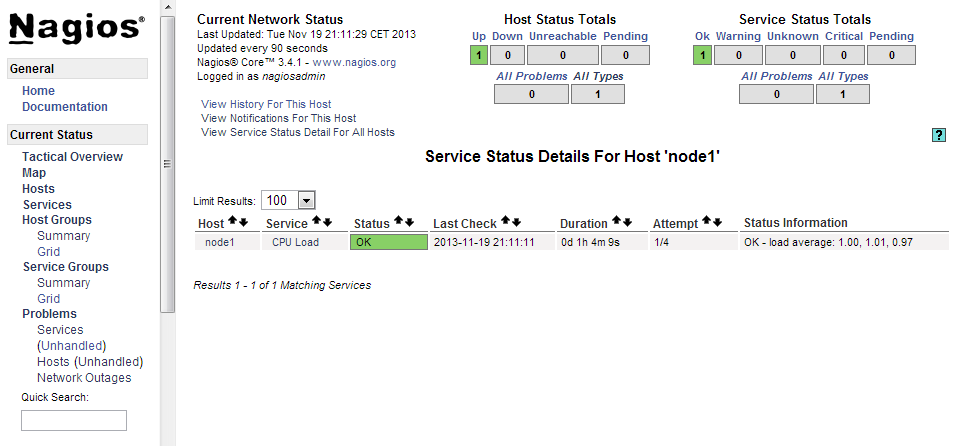
\includegraphics[width=0.5\textwidth]{pics/nagios_2.png}
\end{figure}

TODO:
configuring check\_load arguments: https://kura.io/2010/03/21/configuring-nagios-to-monitor-remote-load-disk-using-nrpe/
which arguments are usefull for checkload:
http://serverfault.com/questions/209566/what-warning-and-critical-values-to-use-for-check-load

To do some more involved tests, I added a new node, which I called
'node2' to my list of virtual machines. I configured this machine in
the same way as I did on 'node1' and added it to the Nagios monitor
server, as described earlier.
This worked without any problems, and Nagios correctly shows the health
and CPU load of both servers 
\cref{fig:nagios_nrpe_also_node2}.

\begin{figure}[h!]
  \caption{Nagios showing both nodes}
  \label{fig:nagios_nrpe_also_node2}
  \centering
    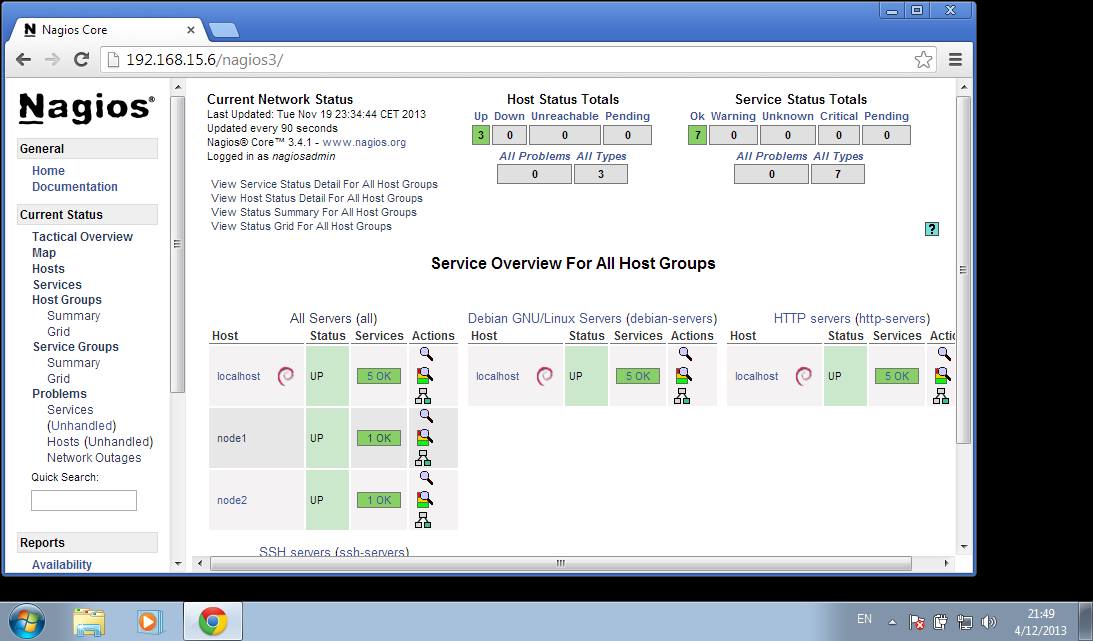
\includegraphics[width=0.5\textwidth]{pics/nagios_3.png}
\end{figure}

Now, let's see how Nagios properly detects system failure. To test
this, we will induce a kernel panic on 'node1'; this can be achieved
by inserting a kernel module that calls the panic() kernel function in
its init function. I found source code to achieve this (src/panic/*)
\cite{simulate_linux_crash}.
To make the kernel crash, first we need to build the module:
\begin{lstlisting}[language=bash]
 make
\end{lstlisting} 
Now we can insert the module into our running kernel:
\begin{lstlisting}[language=bash]
 sudo insmod force_panic.ko
\end{lstlisting} 
This immediately causes a kernel panic \cref{fig:kernel_panic}.
\begin{figure}[h!]
  \caption{'node1' experiencing a kernel panic}
  \label{fig:kernel_panic}
  \centering
    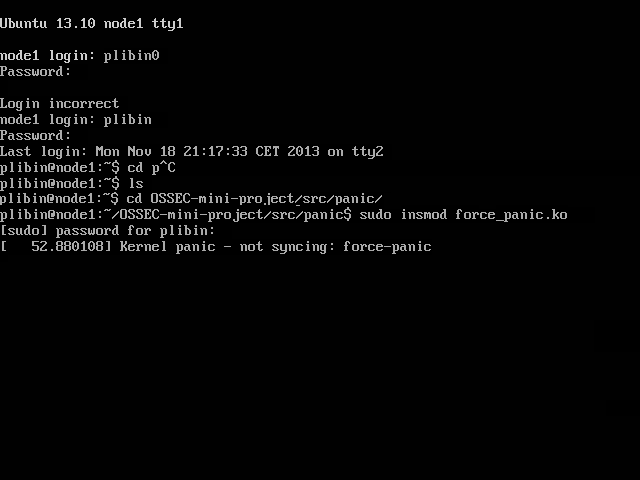
\includegraphics[width=0.5\textwidth]{pics/kernel_panic.png}
\end{figure}
After about one minute, this failure was detected by nagios, and the
user interface depicted a ``Critical error'' \cref{fig:nagios_after_kernel_panic}.

\begin{figure}[h!]
  \caption{Nagios showing a critical error after a kernel panic}
  \label{fig:nagios_after_kernel_panic}
  \centering
    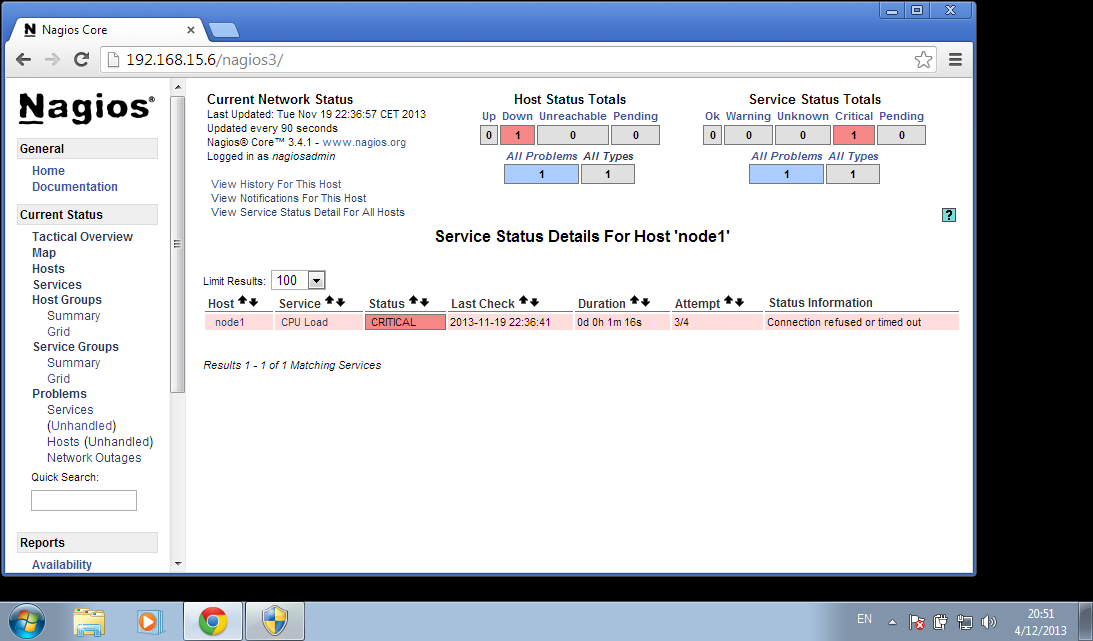
\includegraphics[width=0.5\textwidth]{pics/nagios_after_kernel_panic.png}
\end{figure}

If a node experiences a system failure, it is useful when an action is
performed that tries to solve the problem. An Ubuntu server can be
configured to automatically restart upon a kernel panic
\cite{restart_upon_kernel_panic}, however, when an hardware problem is
the cause of the system crash, restarting the node will be of no
avail. It is better to start a new node, and investigate the problem
on the crashed node in detail.

It is possible to configure an event handler for a Nagios
service. This handler will execute a script on the monitor
server, every time an exceptional event occurs.
For our simulation, we will execute this scenario:
\begin{itemize}
\item crash 'node1'
\item Nagios will notice this crash and an evenhandler will be
  triggered
\item this event handler will send a message to the virtual machine
  controller (in our setup, this is the MacOS X host operating
  system)
\item when the controller receives this message, it will start 'node2'
\end{itemize}
Sending a message will be implemented as writing a file to a shared
directory. This directory has the following layout:
\begin{lstlisting}[language=bash]
 ./nodes/node1
 ./nodes/node2
\end{lstlisting} 
First let's define an eventhandler that places a file named 'crash' in the
shared directory $./nodes/node1/$ whenever Nagios detects a critical
error.
For this to work we need to configure an event handler connected to
the host, we can do this by adding this line to the host definition ($/etc/nagios3/commands.cfg$ ) of 'node1':
\begin{lstlisting}[language=bash]
event_handler   inform-controller
\end{lstlisting} 
We now have to define the $inform-controller$ command:
\begin{lstlisting}[language=bash]
define command {
    command_name    inform-controller
    command_line    /soft/nagios/scripts/inform-controller.sh
$HOSTNAME$ $HOSTSTATE$
}
\end{lstlisting} 
The script inform-controller simply creates a file
$/media/sf\_ossec\_vm\_share/nodes/node1/crash$ whenever Nagios
detects 'node1' goes down.
Find the code for the inform-controller.sh script below:
see: src/inform-controller.sh

Now we need to detect the creation of the file
$/media/sf\_ossec\_vm\_share/nodes/node1/crash$  on the controller,
which is a MacOS X system in my testing environment. On MacOS X, this
can be implemented using ``Folder actions'', with some customized scripts
\cite{folder_actions_bash} it is possible to execute bash scripts when
an file event occurs.
I configured my MacOS X operating system to run this script whenever a
file was added to one of the node directories:

This script will check whether a crash file exists in the $./nodes/node1$
directory, and if this is the case, start 'node2' using VirtualBox's
command line tools. 
Source of the script src/FolderActions.sh

This simple setup shows how Nagios can be used to react on the failure
of cluster nodes. Note that an actual setup might be more
involved; we would for example keep a pool of available systems that
can be started when one of the running cluster nodes fails. In a
cluster environment, our VBoxManage call might be replaced with a
command to direct a hardware controller to power on an available rack
server.

Reference to movie: movies/nagios-setup.mov

\subsection{Ganglia experiment}
I will use the same set of virtual machines to setup the Ganglia
experiment: 'node1', 'node2' and 'monitor'.
The 'monitor' node will periodically ask the client nodes for their
metrics and store these metrics in a round-robin database (see
appendix).
To install the software required for this monitoring (gmetad) we execute the
following command:
\begin{lstlisting}[language=bash]
sudo apt-get install ganglia-monitor gmetad
\end{lstlisting} 

These programs only include the monitoring system, in order to
visualize the results in a web interface we should also install the
web-frontend:
\begin{lstlisting}[language=bash]
sudo apt-get install ganglia-webfronted
\end{lstlisting} 

Ganglia supports 2 modes: multicast (zie appendix) and unicast mode.
Misschien een beetje uitleg over het verschil.
The multicast is the detault mechanism, and is the easiest way to
configure a Ganglia cluster.
For our test setup, where we have an explict monitor server, we will
configure Ganglia using unicast mode.

Let's start by configuring the 'monitor' cluster node. I adapted the
default configuration file that was installed with Ganglia based on an
 installation manual \cite{ganglia_install_manual}.
Here a listing of the most important changes I've made:
src/ganglia\_monitor\_config

The most imporant segments of this configuration listing are:
\begin{itemize}
\item $deaf = no$: the monitor server should listen to the cluster
  nodes
\item cluster name
\item channel (UDP/TCP) configurations
\end{itemize}

To configure the cluster nodes, we only need to install ganglia-monitor:
\begin{lstlisting}[language=bash]
sudo apt-get install ganglia-monitor
\end{lstlisting} 

I adapted the
default configuration file that was installed with Ganglia based on an
 installation manual \cite{ganglia_install_manual}.
Here a listing of the most important changes I've made:
src/ganglia\_node\_config

The most imporant segments of this configuration listing are:
\begin{itemize}
\item $deaf = yes$: the cluster nodes should not listen to other
  cluster nodes, but only send their data to the monitor server
\item cluster name
\item channel (UDP) configuration
\end{itemize}

To finalize the configuration, we need to configure gmetad on
'monitor', we can do this by providing gmetad with this config file
(located at /etc/ganglia/gmetad.conf):
\begin{lstlisting}[language=bash]
data_source "OSSEC" localhost
\end{lstlisting} 

To allow the cluster nodes to send their data to the monitor server,
we still need to open the UDP port $gmetad$ is listening on:
 \begin{lstlisting}[language=bash]
sudo ufw allow 8649/udp
\end{lstlisting} 

OK, let's take it for as spin! When trying to access the web
application, there was a problem, apache was not aware of the ganglia
web application. After copying the ganglia apache configuration to
$/etc/apache2/sites-enabled$, the web application was functional and
show a general overview \cref{fig:ganglia_general}.
\begin{figure}[h!]
  \caption{Ganglia's general overview}
  \label{fig:ganglia_general}
  \centering
    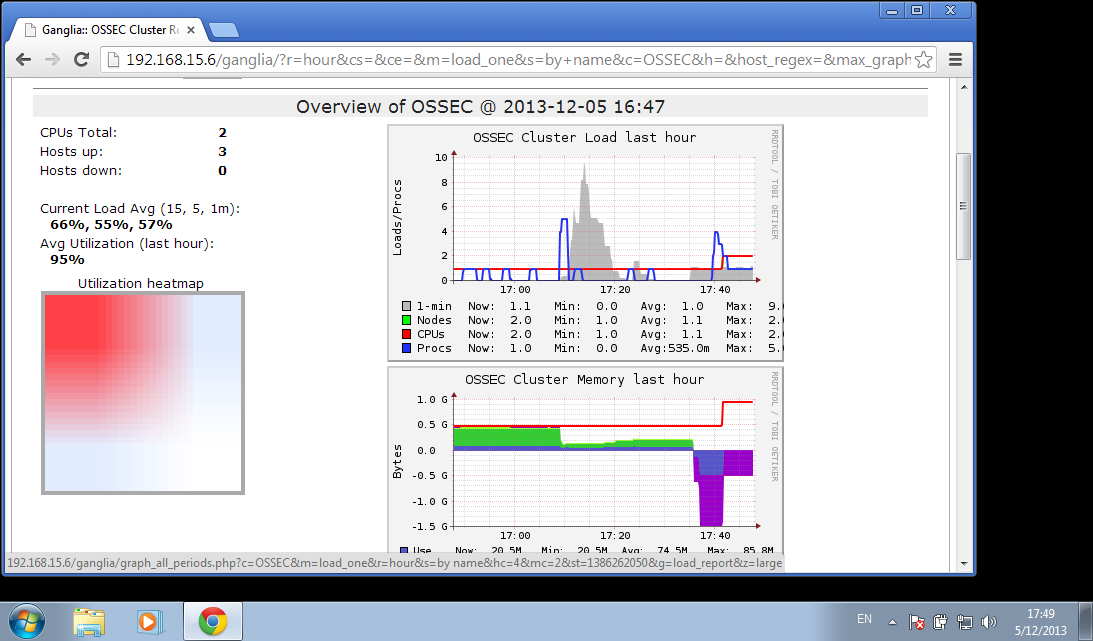
\includegraphics[width=0.5\textwidth]{pics/ganglia_general.png}
\end{figure}
All configured nodes were detected, and an overview of the CPU load of
all 3 nodes was visible on the bottom of the Ganglia's web application
start page  \cref{fig:ganglia_node_overview}.
\begin{figure}[h!]
  \caption{Ganglia's node overview}
  \label{fig:ganglia_node_overview}
  \centering
    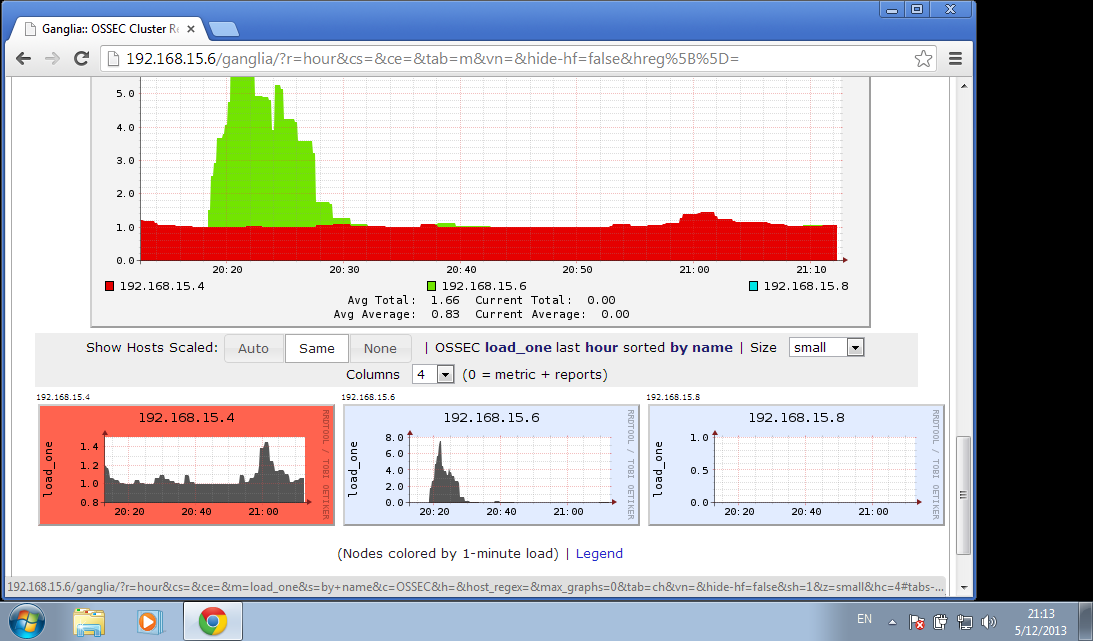
\includegraphics[width=0.5\textwidth]{pics/ganglia_node_overview.png}
\end{figure}
I've started nagios\_app (reference to the previous section) on 'node1'
(IP=192.168.15.4) to put the node under heavy load. This clearly is
visible in the node overview \cref{fig:ganglia_node_overview}.

Since the collected metrics are stored in a round-robin database, it is possible to
extract this data to do research on it. Such research can help
companies to predict/anticipate sudden changes in system load.

All data is stored in $/var/lib/ganglia/rrds/$, for each cluster,
there is a directory. In a cluster directory, each node that belongs
to the cluster has a directory with its name/IP address.
For example: if we want to look at the CPU user-usage of our 'node1',
we need to query this file:
$/var/lib/ganglia/rrds/OSSEC/192.168.15.4/cpu\_user.rrd$. This file is
encoded in a binary format; we can export it to a CSV-file using the
rrd2csv program \cite{rrd2csv}:
\begin{lstlisting}[language=bash]
perl rrd2csv.pl  /var/lib/ganglia/rrds/OSSEC/192.168.15.4/cpu\_user.rrd > node1_cpu_user.csv
\end{lstlisting} 

However, this command will only export the data of the last minute. To
export all data that was collected starting from a point further in time, we need to
explicitely pass the start date in epoch format (see appendix).
An example to extract all data that is one hour old:
\begin{lstlisting}[language=bash]
now = `date +%s`
one_hour_ago = `expr $now - 3600` 
perl rrd2csv.pl -start $one_hour_ago /var/lib/ganglia/rrds/OSSEC/192.168.15.4/cpu\_user.rrd > node1_cpu_user.csv
\end{lstlisting} 

This kind of data can be imported directly by statistical analysis
environments such as R \cite{r_software}.

\subsection{Nagios and Ganglia: conclusions and remarks}
nagios:
pos: 
-event handling -> very powerful
-very extensible + configurable
neg:
-doc is not allways up to date + sometimes incomplete
-difficult installation (largely because of the docs, also because
quite a lot of manual steps were necessary)
ganglia:
pos:
- installation -> easy (apt-get + some config for the unicast mode)
- project doc -> seems ok
- data stored in a round-robin db by default: exist a lot of software
to query/extract/graph data in such databases
neg:
?

both systems very interesting and mostly complementary

\section{HAProxy experiment}
HAProxy is a prominent software load balancer. It acts like a reverse
proxy; pretending it is the main server and then forwarding the
requests to one of the HTTP server cluster nodes.
Several strategies are available to distribute requests over a HTTP
server cluster; these strategies are explained in
\ref{sec:load_balancing_proxies}.
In this experiment, I will setup a HAProxy that sends requests to 2
HTTP server cluster nodes using the 'roundrobin' distribution
strategy.
\subsection{HAProxy installation}
I will install HAProxy on a new Ubuntu virtual machine: 'haproxy'.
I will use the virtual machines 'node1' and 'node2' as HTTP server cluster nodes.
Let's start by properly configuring 'node1' and 'node2' that it can
serve this simple PHP program (from \cite{haproxy_install_tutorial}):
\label{lst:test_php}
\begin{lstlisting}[language=php]
<?php
header('Content-Type: text/plain');
echo "Server IP: ".$_SERVER['SERVER_ADDR'];
echo "\nClient IP: ".$_SERVER['REMOTE_ADDR'];
echo "\nX-Forwarded-for: ".$_SERVER['HTTP_X_FORWARDED_FOR'];
?>
\end{lstlisting} 
This program will print the HTTP server's IP address, the client IP
address (which in our case will be the IP address of our HAProxy
server) and the X-Forwarded-for header (which will allow us to identify
the originating IP adress: i.e. the IP-address of our browser).
First we'll need to install Apache and PHP:
\begin{lstlisting}[language=bash]
sudo apt-get install apache2
sudo apt-get install php5
sudo apt-get install libapache2-mod-php5
sudo /etc/init.d/apache2 restart
\end{lstlisting} 
Now we can copy our test program \ref{lst:test_php} to
$/var/www/test.php$.

Then I opened port 80:
\begin{lstlisting}[language=bash]
  sudo ufw allow 80/tcp
\end{lstlisting} 

After these changes, the nodes were able to serve this PHP test
program: \ref{fig:test_php_working}.

\begin{figure}[h!]
  \caption{Test PHP program working in a browser}
  \label{fig:test_php_working}
  \centering
    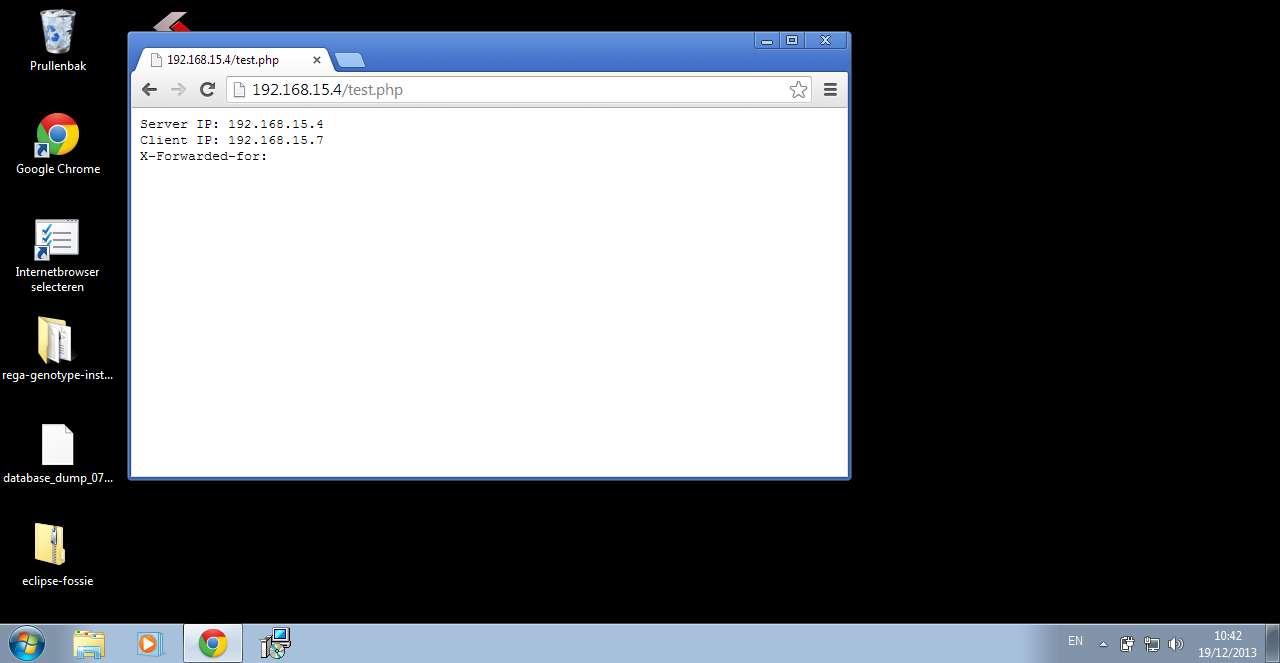
\includegraphics[width=0.5\textwidth]{pics/test_php_working.png}
\end{figure}

To install HAProxy:
\begin{lstlisting}[language=bash]
apt-get install haproxy
\end{lstlisting} 
After this installation, a reboot of the virtual machine was required.
In order to make HAProxy start by the init script we need to put the
ENABLED variable in $/ect/default/haproxy$ to $1$.
I use the HAProxy config file that is installed with the haproxy
Ubuntu package comes with a proper config file by default (reference appendix src/haproxy\_basic.cfg).   
In order to configure HAProxy for a specific application, I conceived
this configuration snippet:
\begin{lstlisting}[language=bash]
listen ossec_app 0.0.0.0:80
        mode http
        balance roundrobin
        option forwardfor
        server node1 192.168.15.4:80 check
        server node2 192.168.15.8:80 check
\end{lstlisting} 
This configuration defines the application ossec\_app on port 80.
I use the 'roundrobin' algorithm, enabled the forwardfor (so we can read
the X-Forwarded-for HTTP header in our PHP test program) and added our 2
HTTP server cluster nodes to the configuration.
Then I opened port 80 on the 'haproxy' server:
\begin{lstlisting}[language=bash]
  sudo ufw allow 80/tcp
\end{lstlisting} 

\subsection{HAProxy testing}
After making the configurations as described in the previous section, I could visit the test PHP program via the
haproxy server (IP address: 192.168.15.10); as demonstrated in \ref{fig:haproxy_working_browser}.

\begin{figure}[h!]
  \caption{Testing the haproxy setup in a browser}
  \label{fig:haproxy_working_browser}
  \centering
    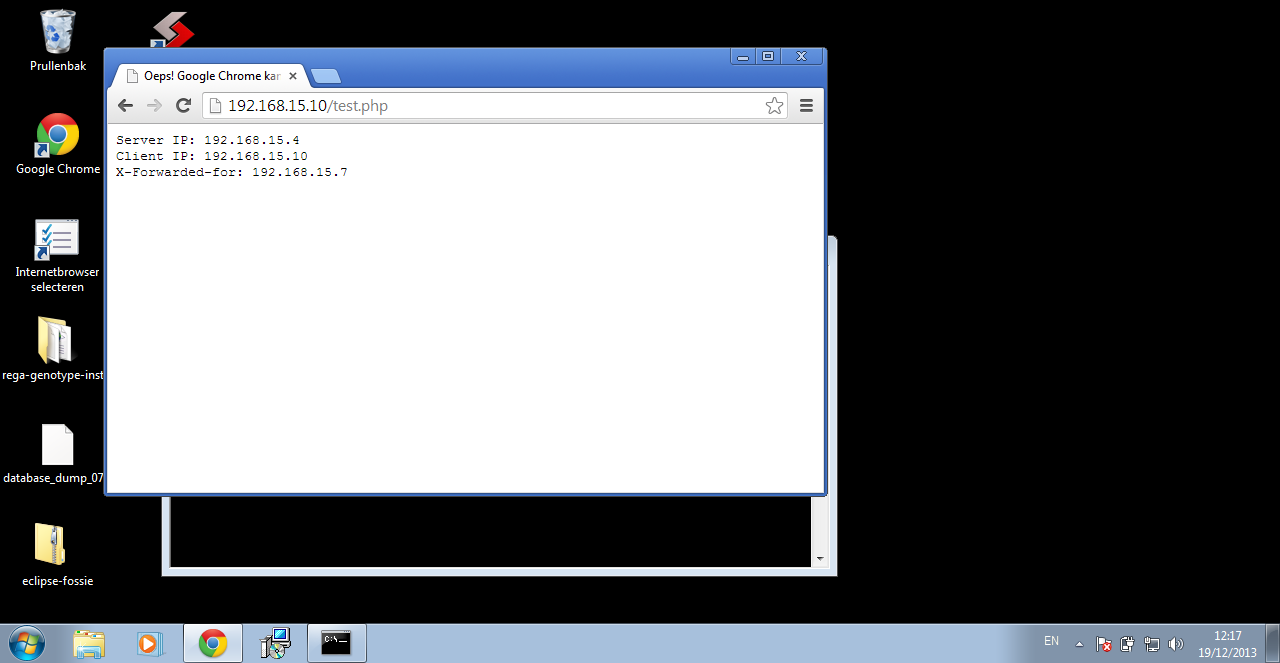
\includegraphics[width=0.5\textwidth]{pics/haproxy_working_browser.png}
\end{figure}

When testing this setup, it becomes clear that HAProxy forwards the
request to both cluster nodes (subsequently to 'node1' and than to
'node2').
I recorded a video to demonstrate this behaviour (reference to
haproxy.mov).

This setup also handles failure of nodes, if we shutdown apache on one
of the nodes, HAProxy will automatically forward the incoming requests
to the working node. 
I recorded a video to demonstrate this behaviour (reference to
haproxy-failover.mov).

\subsection{Conclusion and remarks}
I was able to extract a lot of valuable information from this online
article: \cite{haproxy_install_tutorial}. The online documentation of
 HAProxy \cite{haproxy:2013} is also very good, and explains all
 configuration items in detail, often with some pointers on when an
 how to use them. The documentation for example advices not to use the
 'leastconn' algorithm for HTTP services, since this algorithm is not
 well-suited for services that use short-lived sessions.
The installation went smoothly on Ubuntu, some manual configurations
were necessary, but since the documentation of the project is clear
and up-to-date, this did not cause any problems.

\section{Database replication experiment}
I will setup a master-slave replicated MySQL database. I will use the
'haproxy' virtual machine to act as my master database and I will
install 2 slave databases on my 'node1' and 'node2' virtual machines.
\cite{mysql_official_replication_doc},
\cite{mysql_replication_howtoforge}, 
\cite{mysql_replication_stackexchange}, 

\subsection{Installation} 
I will start by installing mysql (server and client) on all the involved virtual
machines ('haproxy','node1','node2').
\begin{lstlisting}[language=bash]
sudo apt-get install mysql-server mysql-client
\end{lstlisting}

Let's create a test database on our master-node:
\begin{lstlisting}[language=bash]
mysql -u root -p
*type password*
mysql> CREATE DATABASE ossec;
\end{lstlisting}
No we can use this database, and create a simple table in it:
\begin{lstlisting}[language=bash]
mysql> USE ossec;
mysql> CREATE TABLE friend (first_name text, last_name text);
\end{lstlisting}
And we add a friend to it:
\begin{lstlisting}[language=bash]
mysql> INSERT INTO friend (first_name, last_name) values ('Eric',
'Northman');
\end{lstlisting}

The next step is the configuration of the master. Most of the
configuration is done in $/etc/mysql/my.cnf$.
First we need to comment out the bind-address line, this will inform MySQL
to listen on all IP addresses rather than only on localhost:
\begin{lstlisting}[language=bash]
#bind-address        = 127.0.0.1
\end{lstlisting}
MySQL slaves use the logs that a master-node generates to replicate
the database. In order to make this work, we need to tell the MySQL
master-node where to
generate these log files and for which databases the log files need to
be generated. 
\begin{lstlisting}[language=bash]
log-bin = /var/log/mysql/bin.log
#multiple binlog-do-db lines are allowed
binlog-do-db = ossec
\end{lstlisting}
We need to specify the server's id as well, since this is our master
server, we use $id=1$:
\begin{lstlisting}[language=bash]
server-id = 1
\end{lstlisting}
Now we're ready for restarting the database:
\begin{lstlisting}[language=bash]
sudo /etc/init.d/mysql restart
\end{lstlisting}
We need to give a MySQL user (let call him 'reppy') the permission to replicate our
database:
\begin{lstlisting}[language=bash]
mysql -u root -p
*type password*
mysql> GRANT REPLICATIOn SLAVE ON *.* TO 'reppy'@''%' IDENTIFIED BY
                                %'reppy_password';
mysql> FLUSH PRIVILEGES;
\end{lstlisting}
wat doet die percent in de sql code hierboven?

To get the information to configure the slave, we need to execute these
commands to select our database 'ossec' and lock all the tables in it:
\begin{lstlisting}[language=bash]
mysql> USE ossec;
mysql> FLUSH TABLES WITH READ LOCK;
\end{lstlisting}
No we can extract the information we need:
\begin{lstlisting}[language=bash]
mysql> SHOW MASTER STATUS;
\end{lstlisting}
The output of this command is:
\begin{lstlisting}[language=bash]
+---------------+----------+--------------+------------------+
| File          | Position | Binlog_do_db | Binlog_ignore_db |
+---------------+----------+--------------+------------------+
| bin.000003    | 333      | ossec        |                  |
+---------------+----------+--------------+------------------+
1 row in set (0.00 sec)
\end{lstlisting}
Now we need to dump the current database:
\begin{lstlisting}[language=bash]
mysqldump -u root -p --opt ossec > ossec.sql
\end{lstlisting}

It is important to unlock the tables again before we continue:
\begin{lstlisting}[language=bash]
mysql> UNLOCK TABLES;
\end{lstlisting}

To allow the slave nodes to connect to the master database, we need to
open up the MySQL port ($3306$) of the master node:
\begin{lstlisting}[language=bash]
sudo ufw allow 3306/tcp
\end{lstlisting}

Now let's configure the slaves, we start by creating the 'ossec'
database on the slaves:
\begin{lstlisting}[language=bash]
mysql -u root -p
*type password*
mysql> CREATE DATABASE ossec;
\end{lstlisting}
Now we need to apply the dump we obtained on the master server (I
copied the ossec.sql using $scp$):
\begin{lstlisting}[language=bash]
mysql -u root -p ossec < ossec.sql
*type password*
\end{lstlisting}

Next we configure the server-id and the database that is replicated in
$/etc/mysql/my.cnf$:
\begin{lstlisting}[language=bash]
#node 1
server-id = 2 
#node 2
server-id = 3

#same for node 1 and 2
replicate-do-db = ossec
\end{lstlisting}

After these configurations, we need to restart the MySQL server:
\begin{lstlisting}[language=bash]
sudo /etc/init.d/mysql restart
\end{lstlisting}

And execute this SQL to let the slave know where to find its master:
\begin{lstlisting}[language=bash]
mysql> CHANGE MASTER TO MASTER_LOG_FILE='bin.000003',
MASTER_LOG_POS=333, MASTER_HOST='192.168.15.10', MASTER_USER='reppy', MASTER_PASSWORD='reppy_password';
\end{lstlisting}
Now we can start the slave:
\begin{lstlisting}[language=bash]
mysql> START SLAVE;
\end{lstlisting}

\subsection{Testing the experiment setup}
After this, when a change is made to the master database, these
changes are automatically propagated to the slave databases. I
recorded a video to demonstrate this with my test setup (reference
mysql\_replication.mov).

\subsection{Conclusion and remarks}
Setting up a replicated MySQL environment was not easy, mainly since I
had to consult several seperate documents. The main problem seems to
be that the way things are configured in MySQL seems to change significantly
over time. Several settings I found in different tutorials, were no
longer supported on the most recent MySQL package distributed with
Ubuntu.
On the other hand, if something went wrong or behaved unexpectedly,
the output in the log files was quite informative. 
One important remark is that on a slave node, it is no longer possible
to configure the master settings (host, log\_pos, log\_file, user,
password) in the configuration file; you should use the $CHANGE
MASTER ...$ SQL command.

\section{Software disk replication experiment}
I will setup a network RAID-1 (mirroring; appendix: explain RAID-1)
system on 2 nodes, for this I will use the software DRBD 
(Distributed Replicated Block Device) \cite{drbd_soft:2013}.
I will create a disk (virtual machine disk) of 1GB on my virtual
machines 'node1' and 'node2' (since we're using RAID, it is vital that
these disks have the exact same size).

reference: 
http://www.howtoforge.com/setting-up-network-raid1-with-drbd-on-ubuntu-11.10-p2
\cite{drbd_ubuntu_doc}
\cite{drbd_official_doc}

\subsection{Adding the ``disks''}
Firstly, I will add a disk to my virtual machines 'node1' and
'node2'. This can be done via the VirtualBox user interface, when the
virtual machines are powered off \ref{fig:add_disk_vbox}.

\begin{figure}[h!]
  \caption{Added a disk to one of the virtual machines}
  \label{fig:add_disk_vbox}
  \centering
    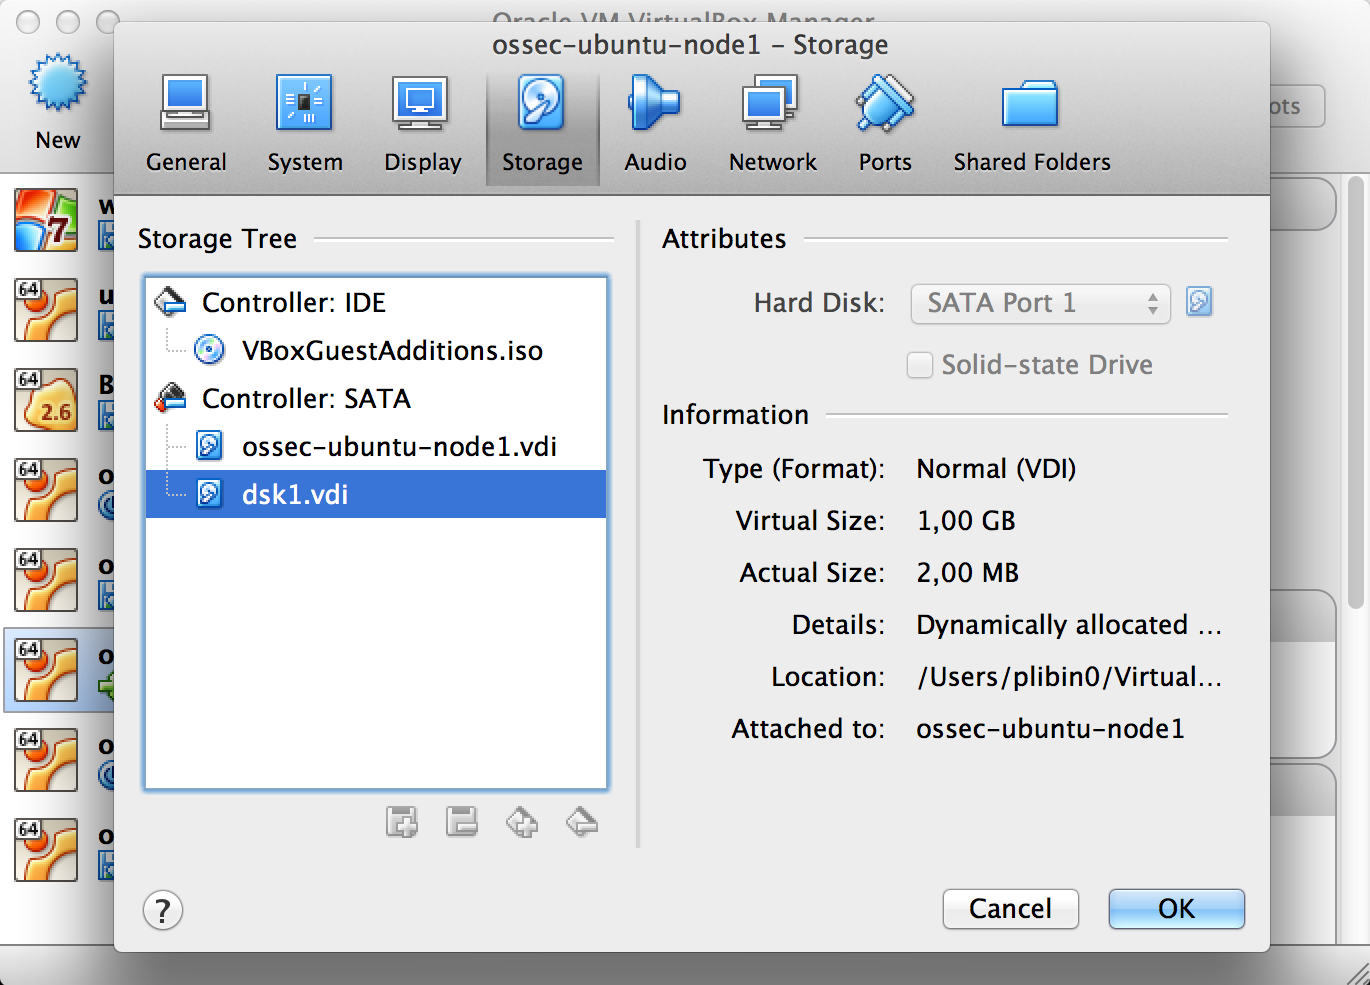
\includegraphics[width=0.5\textwidth]{pics/add_disk_vbox.png}
\end{figure}

\subsection{Setting up the network RAID-1}
To ensure the synchronization is timed well, I will install the NTP
(see appendix) packages.
\begin{lstlisting}[language=bash]
sudo apt-get install ntp ntpdate
\end{lstlisting}

In order for DRBD to work, each node should be able to access the
other node by name. Since we have no DNS in place, we need to
configure this in the $/etc/hosts$ config file.

We added a disk to the virtual machine, however, this disk is
currently an unpartioned and unformatted device.
Let's first have a look at our device:
\begin{lstlisting}[language=bash]
sudo fdisk -l /dev/sdb
\end{lstlisting}
This command show the following report:
\begin{lstlisting}[language=bash]
out/fdisk-l.txt
\end{lstlisting}
To create a partion:
\begin{lstlisting}[language=bash]
sudo fdisk /dev/sdb
Command (m for help): n #create a new partition
Select (default p): p #primary parition
Partition number (1-4, default 1): 1
First sector (2048-2097151, default 2048): 2048
Last sector (2048-2097151, default 2097151): 2097151
\end{lstlisting}
The partition is created, but we still need to write the partition
table to the disk:
\begin{lstlisting}[language=bash]
Command (m for help): w #write the partition table to disk
\end{lstlisting}
When running $fdisk -l$ again, we get this output:
\begin{lstlisting}[language=bash]
out/fdisk-l-2.txt
\end{lstlisting}

Now we need to install the DRBD utilities:
\begin{lstlisting}[language=bash]
sudo apt-get install drbd8-utils
\end{lstlisting}
And load the DRBD kernel module:
\begin{lstlisting}[language=bash]
sudo modprobe drbd
\end{lstlisting}

We can configure these nodes with the following configuration file
(based on: \cite{drbd_ubuntu_doc} \cite{drbd_official_doc}):
\begin{lstlisting}[language=bash]
src/drbd/drbd.conf
\end{lstlisting}
Most of the configuration items are straightforward, I commented the
other elements to clarify their meaning.
The configuration file should be placed in $/etc/drbd.conf$.

We need to open the ports 7789 on both nodes:
\begin{lstlisting}[language=bash]
sudo ufw allow 7789/tcp
\end{lstlisting}

We also need to restart the drbd daemon: 
\begin{lstlisting}[language=bash]
sudo /etc/init.d/drbd restart
\end{lstlisting}

First I started the daemon on 'node1', the daemon waited untill the
daemon I brought the daemon on 'node2' online.

\subsection{Conclusions and remarks}
When starting the drdb service, you need to specify
whether you want the software to send statistics (anonymized) to a
server of the DRBD organization. -> not sure what to think about this
To disable this, we need to add the line $usage-count no;$ to the config file's
global section.
I recorded a short video that demonstrates this: start\_drbd.mov.

Now we configured the mirrored device $/dev/drbd0$, but we can't use
this device yet.
We first need to initialize the meta data storage of each physical
device,
one both nodes, we need to run this command:
\begin{lstlisting}[language=bash]
sudo drbdadm create-md r0
\end{lstlisting}
We also need to decide which node will be the primary node; on this
node we will be able to read and write data d.
For now, I will make 'node1' the primary node for this device.
First we need to invalidate the data on 'node2', so BRBD knows this
data can safely be overriden; we use this command:
\begin{lstlisting}[language=bash]
sudo drbdadm invalidate r0
\end{lstlisting}
To make the device on 'node1' the primary divice,
we need to run this command on 'node1':
\begin{lstlisting}[language=bash]
sudo drbdadm --force primary r0
\end{lstlisting}
Now the device on 'node1' gets automatically synched with the one on
'node2'. But there doesn't exist a filesystem on our device yet; let's
create an ext3-filesystem (this command is executed no 'node1'):
\begin{lstlisting}[language=bash]
sudo mkfs.ext3 /dev/drbd0
\end{lstlisting}
Now we can mount the filesystem (on 'node1'):
\begin{lstlisting}[language=bash]
sudo mkdir /media/drdb0
sudo mount /dev/drbd0 /media/drbd0 
\end{lstlisting}
To test that the replication actually works, we need to:
\begin{itemize}
\item create some files on $/media/drbd0$ on 'node1'
\item unmount the $/media/drbd0$ on 'node1'
\item make 'node1' the secondary host
\item make 'node2' the primary host
\item mount the device on 'node2'
\item check that the files we placed on the device from 'node1' also
  appear on 'node2'
\end{itemize}
I created a video to demonstrate and test this scenario:
test\_drbd.mov.

\subsection{Conclusions and remarks}
When starting the drdb service, you need to specify
whether you want the software to send statistics (anonymized) to a
server of the DRBD organization. -> not sure what to think about this
To disable this, we need to add the line $usage-count no;$ to the config file's
global section.
The online documentation on how to configure the software is
up-to-date and helpful. It is a nice and interesting software, that easily allows you
to setup replication between datacenters on blocklevel.

\section{Distributed file system experiment}
I will experiment with Ceph, since this seems to be the de-facto
standard distributed filesystem in the Ubutu landscape.
Except for better compatibility with Ubuntu, there is no real reason
to choose Ceph over GlusterFS; both seem to be decent projects
\cite{ceph_vs_gluster_1}, \cite{ceph_vs_gluster_debate}.
Ceph is a large project, with many features: object storage, file
system, block device layer, ... In this experiment, I will focus on
the distributed file system component.

\subsection{Architecture}
\label{subsec:ceph_architecture}
Discuss architecture: 
\begin{itemize}
\item developerWorks article (printed):
  http://www.ibm.com/developerworks/library/l-ceph/
\item http://www.anchor.com.au/wp-content/uploads/2012/09/ceph\_stack.png
\end{itemize}

\subsection{Installation}
Ceph can be installed in 2 ways: via ceph-deploy (as piece of software
that is installed on an administrator node that automatically installs the
necessary components on the nodes in your Ceph cluster) and a
manual installation.
The advantages of the first approach:
\begin{itemize}
\item quicker to setup
\item commands entered on the administrative node are 
  propagated to all relevant cluster nodes (this makes upgrading nodes
  much easier)
\end{itemize}
The main advantage of a manual installation is that it allows you to
fully control where and when all necessary components are installed on the different
nodes. 
This might be interesting on a production cluster, however I think the
installation via ceph-deploy is more appropriate for this experiment, since it will
allow me to test more of Ceph's features in a shorter timespan.

\subsubsection{Nodes}
We will first setup a cluster with 1 administrator node and a Ceph
Storage Cluster consisting of 3 cluster nodes (this setting is adviced
by the official documentation to experiment with the software \cite{ceph_official_doc}).
For this, I create 4 new clones of my base virtual machine:
'ceph-admin', 'ceph-node1', 'ceph-node2', 'ceph-node3'.

\subsubsection{Preparation of the cluster nodes}
Ceph requires some basic stuff to be in place, in order to be able to
use ceph-deploy to configure the cluster and cluster nodes.
The instructions are well documented in the official documentation's
``Ceph node setup'' section \cite{ceph_official_doc}.
A quick overview of the different steps:
\begin{itemize}
\item create a 'ceph' user on each node
\item add root privileges to the 'ceph' user
\item install an ssh server
\item configure the admin node so that it can access the cluster nodes
  without using a password (using SSH keys)
\item all nodes should be able to access each other using hostname
  resolution, in my case, we had to update the $/etc/hosts$ file to
  make this possible, since we have no DNS server in our lab setting
\end{itemize}

\subsubsection{Configuring the ceph-admin node}
The documentation requests to add the ceph-deploy package to your
local APT
repository, however on Ubuntu 13.10, this package was already
available by default.
So we can install it like this:
\begin{lstlisting}[language=bash]
sudo apt-get install ceph-deploy
\end{lstlisting}
We also need to create a directory to maintain the configuration of
our cluster (the name is not important, but we will use
~/ossec-cluster consistently through the example for clarity):
\begin{lstlisting}[language=bash]
mkdir ~/ossec-cluster
\end{lstlisting}
It is important that we run  the ceph-deploy command in this
directory, since it will export its output to the current directory.

\subsubsection{Setting up the cluster}
Now we can start configuring our cluster \footnote{The following steps are executed on the 'ceph-admin'}.
We will configure 'ceph-node1' as a monitor node, 'ceph-node2' and
'ceph-node-3' will be object storage daemons \ref{subsec:ceph_architecture}.

cite ceph documentation

To start a new cluster with monitor node 'ceph-node1':
\begin{lstlisting}[language=bash]
cd ~/ossec-cluster
ceph-deploy new ceph-node1
\end{lstlisting}
After executing these commands, a set of files will be created in
~/ossec-cluster.
To install ceph on our nodes:
\begin{lstlisting}[language=bash]
ceph-deploy install ceph-node1 ceph-node2 ceph-node3
\end{lstlisting}
Every Ceph cluster is required to have at least one monitor
\footnote{Multiple monitor nodes are also supported; this is vital for a high
  availability production cluster, but outside the scope of this experiment} :
\begin{lstlisting}[language=bash]
ceph-deploy mon create ceph-node1
\end{lstlisting}
To be able to add Object Storage Daemons, we need to gather the
monitor node's
keys:
\begin{lstlisting}[language=bash]
ceph-deploy gatherkeys ceph-node1
\end{lstlisting}
To add the Object Storage Daemons (OSDs), we first need to make a uniquely
named directory on the nodes. I created /opt/OSD-disk0 on ceph-node2 and
/opt/OSD-disk1 on ceph-node3. 
Now we can prepare and activate the OSDs:
\begin{lstlisting}[language=bash]
ceph-deploy osd prepare ceph-node2:/opt/OSD-disk0 ceph-node3:/opt/OSD-disk1
ceph-deploy osd activate ceph-node2:/opt/OSD-disk0 ceph-node3:/opt/OSD-disk1
\end{lstlisting}

In order to use the ceph command line tool without the need to specify
the monitor address, we need to copy the configuration and admin key
to all nodes.
This goes as advertised in the documentation for the cluster nodes:
\begin{lstlisting}[language=bash]
ceph-deploy admin ceph-node1 ceph-node2 ceph-node3 
\end{lstlisting}
However, this does not work for the administrator node; apparently
this is caused by a bug \cite{ceph_bug_1} that results in the fact
that no config file is written to /etc/ceph.
We can circomvent this problem by first copying the config files that
reside in ~/ossec-cluster to /etc/ceph and than running ``ceph-deploy
admin''.
In order to make sure the correct config file is written to /etc/ceph,
we need to specify the option ``--overwrite-conf''.
This full set of commands:
\begin{lstlisting}[language=bash]
sudo cp -R ~/ossec-cluster /etc/ceph
ceph-deploy admin --overwrite-conf ceph-admin
\end{lstlisting}

\subsubsection{Testing our cluster}
Now, we have setup the cluster properly, we can control the cluster
with the ``ceph'' command, to install this command run: 
\begin{lstlisting}[language=bash]
sudo apt-get install ceph-common
\end{lstlisting}
First let's check the status of our cluster:
\begin{lstlisting}[language=bash]
ceph health
\end{lstlisting}
Executing this command should return ``HEALTH\_OK''.

I recorded a short video that shows the different cluster nodes and
lists the monitor and OSD nodes using the 'ceph' command: ceph\_cluster.mov.

To store and retrieve an object to our cluster, we can do this with
the rados tool \ref{subsec:ceph_architecture}. This tool allows us to
read/write objects respectively from/to a pool.
Pools can be created and removed with the rados tool, when setting up
the cluster, three pools are created automatically: data, metadata,
rbd.
To store a file to the default data pool, we can use the following
commands:
\begin{lstlisting}[language=bash]
echo "Dear Diary, today I played with Ceph..." > diary.txt
rados put diary-text-obj diary.txt --pool=data
\end{lstlisting}
To view what is in the data pool, we can use this command:
\begin{lstlisting}[language=bash]
rados --pool=data ls
\end{lstlisting}
We can also request the ``physical'' location of our file, the
so-called placement group \ref{subsec:ceph_architecture}:
\begin{lstlisting}[language=bash]
ceph osd map data diary-text-obj
\end{lstlisting}
Note that this location may change as our cluster's design changes
(OSD's that are added, or removed).
To get our precious diary back:
\begin{lstlisting}[language=bash]
rados get diary-text-obj -o diary.txt --pool=data
\end{lstlisting}
I recorded a video that demonstrates these commands: ceph\_test.mov

\subsubsection{Adding OSDs on the fly}
It is possible to add OSDs on the fly, to increase capacity for
example. When an OSD is added the cluster will automatically be
rebalanced.
Adding OSDs is done in the same way as I approached earlier,
to add a OSD on 'ceph-node1' we need to execute this code:
\begin{lstlisting}[language=bash]
ceph-deploy osd prepare ceph-node1:/opt/OSD-disk2
ceph-deploy osd activate ceph-node1:/opt/OSD-disk2
\end{lstlisting}

\subsubsection{Setting up the Ceph FileSystem}
In order to setup the file system ... need to install something
more...
simply goes on top of the Cluster Storage system

\subsection{Conclusion and remarks}
ceph or glusterfs: seems to be pretty much the same, ceph backed by
ubuntu, maybe easier to  configure on ubuntu?
security: root ceph user???
ceph-deploy install -> works very well, quite impressive
Because of the bug I ran into \cite{ceph_bug_1}, I had to redo the
installation quite a few time, to figure out a solution for the
problem.
It is good to now that you can undo all installation residues with the
following commands:
\begin{lstlisting}[language=bash]
sudo cp -R ~/ossec-cluster /etc/ceph
ceph-deploy purge ceph-admin ceph-node1 ceph-node2 ceph-node3
ceph-deploy purgedata ceph-admin ceph-node1 ceph-node2 ceph-node3
ceph-deploy forgetkeys ceph-admin ceph-node1 ceph-node2 ceph-node3
\end{lstlisting}
Note that the purge command is not mentioned in the documentation, but
this seems to be important as well!
Of course it would be nice that the installation procedure did not have any bug
at all; however knowing that you can safely screw thing up and return to a
clean slate, is quite comforting.
Very powerfull software
remarkably easy to setup
clean architecture (different layers)
able to configure what is important, redundance, speed to read/write 
possibility to make snapshots
Although this software does a lot of things (nicely seperate libraries
per layer), since it is open source software, it is still possible to
review what is going on.

\section{Database Shards}
Hortizontal scaling in RDBMs is quite involved, their are different
aspects to it; managing shards, propagating queries to shards,
inserting data into new shards.
I did some reseach into existing solutions for MySQL and Postgres, but
I was not able to find a solution that properly covers all the
aforementioned aspects and that would fit in the scope of this
experiment.
Some of the solutions that I picked up that looked quite interesting:
\begin{itemize}
\item vitesse cite
\item cubrid
\item MySQL NDB cluster
\item pgPool
\end{itemize}

\chapter{Creating a `Wikpedia clone' cluster}
interesting hints to improve performance: Tarreau:2006 article: p
17-18 (printed)

\chapter{Conclusion} % Major section
\section{What is lacking}
The ability to replicate journaled filesystems (by using the journal),
like in MS DPM.

\begin{appendices}
\chapter{Concepts}
Round robin (refer to this appendix from the places where round robin
was used)
Round robin database
ACID
RAID
RAID-1
delta encoding
NTP
HMAC
\end{appendices}

%----------------------------------------------------------------------------------------
%	BIBLIOGRAPHY
%----------------------------------------------------------------------------------------



\bibliography{mybib}{}
\bibliographystyle{ieeetr}

%----------------------------------------------------------------------------------------

\end{document}
